\documentclass[conference]{IEEEtran}
\IEEEoverridecommandlockouts
\usepackage[T1]{fontenc}
\usepackage[utf8]{inputenc}
\usepackage{amsmath,amssymb}
\usepackage{graphicx}
\usepackage{booktabs}
\usepackage{multirow}
\usepackage{array}
\usepackage{url}
\usepackage[hidelinks]{hyperref}
\usepackage{cite}

\begin{document}

\title{Predicting Annual Dropout Rates of Colombian Higher-Education Institutions from Open Data: Persistence, Cold Start and the Limits of Context}

\author{\IEEEauthorblockN{Miguel \'Angel M\'endez Rodr\'iguez}
\IEEEauthorblockA{\textit{Maestr\'ia en Inteligencia Artificial y Ciencia de Datos} \\
\textit{Universidad Aut\'onoma de Occidente}\\
Cali, Colombia}
}

\maketitle

\begin{abstract}
We study whether the annual dropout rate of Colombian higher-education institutions (HEIs) can be predicted from open data. We built our own institution-year panel by an ETL process over four public sources (SPADIES, SNIES, Saber~11 and TerriData): 1,928 rows, 295 HEIs, 2015--2021, with lagged features and documented quality filters. We frame two tasks. In Task~1, forecasting with the institution's own history, last year's rate (a naive persistence baseline, MAE 0.0256) is almost unbeatable: only a ridge model that corrects the naive forecast improves it, by about 4\% (corrected $t$-test $p=0.011$ after nested tuning), a gain that loses significance without Bogot\'a or with fewer years, and no model is distinguishable from it in a pre-pandemic or pandemic temporal split. In Task~2, cold-start estimation from institutional and territorial context alone, no combination of three models (ridge, random forest, XGBoost) and three preprocessing methodologies (target transform, imputation, dimensionality reduction including kernel PCA, an autoencoder and K-means cluster features) beats the median by institution type and sector (MAE 0.0405) after correcting for fold dependence. Evaluation uses grouped, repeated cross-validation with the Nadeau--Bengio corrected $t$-test, nested hyperparameter search, temporal splits and municipality-level cold start. The results suggest that institutional dropout is highly persistent and that public territorial context adds no detectable predictive value beyond institution type.
\end{abstract}

\begin{IEEEkeywords}
student dropout, higher education, open data, ETL, regression, cross-validation, cold start, Colombia
\end{IEEEkeywords}

\section{Introduction}

Student dropout is costly for everyone involved. The student loses years of study and future income; families and the State lose what they invested in tuition, loans and subsidies. In Colombia, the annual dropout rate of the higher-education system was 8.97\% in 2023 and 9.78\% in 2024 according to the Ministry of Education's SPADIES system~\cite{men_spadies}, and cohort dropout is far higher: 36.7\% of the students who started in 2016 had dropped out after ten semesters~\cite{lee74}. The rate is also very uneven: in our panel it ranges from 4.3\% to 26\% between the 5th and 95th percentiles of institutions.

Public information on dropout is retrospective. SPADIES reports an institution's rate after dropout has happened, and there is no public, forward-looking estimate per institution. Most of the machine-learning literature predicts dropout for individual students, using either one public dataset from a single Portuguese institution~\cite{realinho2022} or internal records that cannot be shared or replicated (Section~\ref{sec:related}). Resources for retention, however, are allocated by institution and territory, and Colombia publishes no open student-level data.

We therefore pose dropout prediction at the institution level, as a supervised regression on an institution-year panel built only from open data. Early experiments showed that the problem splits naturally into two tasks with different answers:
\begin{itemize}
\item \textbf{Task 1, forecasting with history.} Predict an institution's rate in year $t$ when its past rates are known. The natural baseline is persistence: last year's rate.
\item \textbf{Task 2, cold-start estimation.} Predict the rate from institutional and territorial context alone, as for a new institution, a new campus, or an institution whose reported history is unreliable. The baseline is the median rate of institutions of the same type and sector.
\end{itemize}

Our contributions are:
\begin{enumerate}
\item A reproducible ETL that builds an institution-year dataset (1,928 rows, 295 HEIs, 2015--2021) from four Colombian open sources, with explicit lags, quality filters, 448 automated tests with continuous integration, a single-command reproduction, a measured bias analysis, and an installable package whose command-line interface trains and applies the final models, documented in a model card~\cite{mitchell2019}.
\item A rigorous evaluation protocol: grouped cross-validation by institution, repeated $5\times5$ with the Nadeau--Bengio corrected $t$-test~\cite{nadeau2003}, a two-stage screening/confirmation design, nested hyperparameter search, temporal splits and a municipality-level cold start.
\item A comparison of three models and three preprocessing methodologies, including nonlinear dimensionality reduction (kernel PCA, an autoencoder) and K-means cluster features.
\item An honest negative result: persistence dominates Task~1, and territorial context adds no detectable value over institution type in Task~2.
\end{enumerate}

\section{Related Work}\label{sec:related}

Almost all machine-learning work on dropout predicts it for individual students, and most of it reuses one dataset or private records. Table~\ref{tab:lit} summarizes the open-access studies we reviewed.

\begin{table}[!t]
\caption{Reviewed studies: all predict at the student level}
\label{tab:lit}
\centering\footnotesize
\begin{tabular}{@{}>{\raggedright\arraybackslash}p{0.7cm}>{\raggedright\arraybackslash}p{3.0cm}>{\raggedright\arraybackslash}p{3.9cm}@{}}
\toprule
Study & Data and unit & Models and main result \\
\midrule
\cite{realinho2022} & 4,424 students, one Portuguese HEI (UCI) & Dataset descriptor; basis of most later studies \\
\cite{villar2024} & Same UCI dataset & LightGBM, CatBoost, RF, LR; boosting wins \\
\cite{hoyos2023} & First-semester students, UTP (Colombia) & Logistic regression with SMOTE \\
\cite{gutierrez2021} & Students of one HEI in Bogot\'a & PCA and K-means; economic causes dominate \\
\cite{andrade2023} & Systematic review (PRISMA) & Random forest is the most used model \\
\cite{perez2024} & Review, higher education & Tree ensembles dominate \\
\bottomrule
\end{tabular}
\end{table}

Three gaps follow from this literature. First, the unit of analysis is the student of a single institution; no study predicts institution-level rates across a national system. Second, the data are either the same public dataset or internal records that cannot be replicated. Third, evaluation usually relies on random row splits and accuracy, which overstate performance when rows of the same entity appear in training and test.

We address the three gaps with a national institution-year panel built from open data, validation grouped by institution and by time, and statistical tests that account for the dependence between cross-validation folds~\cite{nadeau2003}. On methods, we follow common practice in the reviewed work (regularized linear models, random forests and gradient boosting~\cite{pedregosa2011,chen2016}) and add nonlinear dimensionality reduction, kernel PCA~\cite{scholkopf1998} and autoencoders~\cite{hinton2006}, as alternatives to PCA.

\section{Dataset Construction}

The final dataset has 1,928 institution-year rows for 295 HEIs, with target years 2015--2021 and 43 columns. Every step is code in the public repository~\cite{repo}, and a test suite of 448 checks, run by continuous integration, covers the ETL and the modeling code. A single command reruns every stage; from a clean clone, the ETL regenerates the dataset byte for byte (same SHA-256), and the seeded experiments reproduce the published results exactly.

\subsection{Sources}
\begin{itemize}
\item \textbf{SPADIES (Ministry of Education):} dropouts and enrolled students per semester for 343 HEIs, 1998--2024; it provides the target and the history features.
\item \textbf{SNIES (Ministry of Education):} the HEI catalog, sector (public or private), character (technical, technological, university institution, university), main-campus municipality, and program-level enrollment from 2015.
\item \textbf{Saber 11 (ICFES):} scores and socioeconomic profile of high-school graduates, aggregated by municipality.
\item \textbf{TerriData (National Planning Department):} 1,102 municipalities, with population, education coverage, poverty and municipal performance.
\end{itemize}
All sources are joined through the DIVIPOLA municipality code of the main campus.

\subsection{Target and Lags}
We use the official SPADIES definition: the dropout rate of semester $t$ is the number of dropouts in $t$ divided by students enrolled two semesters earlier, and the annual rate weights the two semesters of a year. To avoid leakage, context features are lagged one year ($t-1$) and enrollment two semesters ($t-2$). Census 2018 indicators enter only from target year 2020, after their publication, and population enters only in relative terms because the census base changed. A test recomputes 55,813 feature values from their sources with the allowed lag and finds no discrepancy.

\subsection{Quality Filters}
Rows with unreliable targets are removed before modeling (220 of 2,148 institution-years, 10.2\%); Section~\ref{sec:prep} details these filters as the first preprocessing step.

\subsection{Exploratory Analysis}
The median annual rate is 9.9\% (mean 12.0\%, 95th percentile 26.1\%). The rate falls with institution size (Spearman $\rho=-0.36$), and its spread is 5.7 to 14.6 times what binomial noise would produce, so the variation between institutions is real and heteroscedastic. Technical and technological institutions have the highest and most dispersed rates (medians 13.7\% to 20.6\%). Missing values occur in year blocks (municipal performance and SNIES in 2015--2016, Saber~11 in 2019 and 2021), equally in public and private HEIs. Section~\ref{sec:bias} reports the bias analysis.

\section{Data Preprocessing}\label{sec:prep}

Preprocessing follows three methodologies: cleaning, normalization and encoding, and feature selection and extraction (Table~\ref{tab:prep}). Cleaning is applied once to the dataset; every other step is fitted only on the training part of each cross-validation fold and then applied to its test part, so no information from test institutions reaches the model.

\begin{table}[!t]
\caption{The three preprocessing methodologies and the options compared}
\label{tab:prep}
\centering\footnotesize
\begin{tabular}{@{}>{\raggedright\arraybackslash}p{1.9cm}>{\raggedright\arraybackslash}p{3.3cm}>{\raggedright\arraybackslash}p{2.6cm}@{}}
\toprule
Methodology & Options & Fitted on \\
\midrule
1. Cleaning & Quality filters, special-regime exclusion, missingness flags, $\log(1+x)$ of enrollment & Whole dataset (rule-based) \\
2. Normalization and encoding & Median or KNN imputation; standardization; one-hot sector and character; target untransformed or logit & Training fold \\
3. Feature selection and extraction & None, mutual information, PCA, kernel PCA, autoencoder; optional K-means features & Training fold \\
\bottomrule
\end{tabular}
\end{table}

\subsection{Cleaning}
Four filters remove institution-years whose target cannot be trusted: fewer than 100 enrolled students in the denominator, where a handful of dropouts moves the rate by several points (97 rows); SPADIES and SNIES enrollment that disagree by a factor above 3 (37 rows); likely closure (9 rows); and special-regime institutions, mainly military and police schools, whose enrollment rules differ (77 rows). The national training service (SENA) is kept and flagged. Missing values occur in year blocks, so each block gets a binary indicator (missing Saber~11, municipal performance or SNIES data) that lets the model separate ``not published'' from a real value. Enrollment, which spans three orders of magnitude, enters as $\log(1+x)$.

\subsection{Normalization and Encoding}
Numeric features are imputed with the training median or with KNN ($k=5$), then standardized to zero mean and unit variance with the training statistics, so that ridge penalizes all coefficients on the same scale. Sector and character are one-hot encoded. The target, a proportion bounded in $(0,1)$ and right-skewed, is modeled either directly or through the logit transform $\log\frac{y}{1-y}$, with predictions mapped back by the inverse transform.

\subsection{Feature Selection and Extraction}
Five options reduce or reshape the encoded inputs: none; selection of the 15 features with the highest mutual information with the target; PCA keeping 90\% of the variance; kernel PCA with an RBF kernel and the same number of components~\cite{scholkopf1998}; and an autoencoder $n\to16\to8\to16\to n$ trained with early stopping, whose 8-unit bottleneck replaces the inputs~\cite{hinton2006}. Independently, K-means ($k$ chosen by silhouette between 3 and 8) can add the cluster label and the distances to each centroid as new features. LDA is not used: it is a supervised linear method for classes and would require discretizing the continuous rate.

\section{Methodology}

\subsection{Task 1: Forecasting with History}
History features are the rates of $t-1$ and $t-2$, the mean of all previous rates (back to 1999) and the number of previous years, plus a flag for rows without history. We compare two formulations against the naive forecast $\hat y_{i,t}=y_{i,t-1}$: \textbf{B}, direct prediction of the rate from history, with or without context; and \textbf{C}, correction of the naive forecast,
\begin{equation}
\hat{y}_{i,t} = y_{i,t-1} + f(\mathbf{x}_{i,t}), \quad f \text{ trained on } y_{i,t}-y_{i,t-1}.
\end{equation}
A conservative variant drops the $t-1$ rate, in case it is not yet published when year $t$ starts, and is compared with a lagged naive forecast (rate of $t-2$).

\subsection{Task 2: Cold-Start Estimation}
The model sees only context: 33 numeric features (institution size, municipal Saber~11 scores, coverage, poverty, municipal performance, missingness flags) and two categorical ones (sector and character). No history feature is allowed. Baselines are the training median and the training median by character $\times$ sector.

\subsection{Models}
We compare three models of increasing flexibility: ridge regression, a regularized linear model; random forest, an ensemble of decision trees on bootstrap samples; and XGBoost, gradient-boosted trees~\cite{pedregosa2011,chen2016}. Every model is crossed with every preprocessing option of Section~\ref{sec:prep}, which yields 120 configurations in Task~2.

\subsection{Validation and Statistical Tests}
All splits are grouped by institution, so a test institution is never seen in training. Task~2 uses two stages so that selection and confirmation do not share folds: a screening of the 120-configuration grid with one 5-fold split, then a confirmation of the best configuration of each model and of each reduction method with $5\times5$ repeated grouped CV and new seeds. The 25 fold scores are not independent, so confidence intervals and $p$-values use the corrected variance of Nadeau and Bengio~\cite{nadeau2003},
\begin{equation}
\hat{\sigma}^2_{\mathrm{corr}} = \left(\frac{1}{J} + \frac{n_{\mathrm{test}}}{n_{\mathrm{train}}}\right) s^2, \quad J=25,\ \frac{n_{\mathrm{test}}}{n_{\mathrm{train}}}=0.25.
\end{equation}
We also report the Wilcoxon signed-rank test, which ignores this dependence and is therefore optimistic, and a Bonferroni correction. A model \emph{beats} its baseline only when both tests give $p<0.05$. The metric is MAE in rate units; RMSE and $R^2$ are in the repository.

\section{Results: Task 1 (Forecasting with History)}

Persistence dominates. Repeating last year's rate gives MAE 0.0256, and only one of eight pre-registered configurations beats it in both tests (Table~\ref{tab:t1}, Fig.~\ref{fig:t1}).

\begin{table}[!t]
\caption{Task 1: $5\times5$ grouped CV, default hyperparameters}
\label{tab:t1}
\centering\footnotesize
\setlength{\tabcolsep}{3pt}
\begin{tabular}{@{}lcrcc@{}}
\toprule
Configuration & MAE [95\% CI] & Impr. & $p_W$ & $p_t$ \\
\midrule
Naive (rate of $t-1$) & 0.0256 [0.0207, 0.0305] & -- & -- & -- \\
Lagged naive ($t-2$) & 0.0311 [0.0255, 0.0366] & $-21.3\%$ & $<.001$ & $<.001$ \\
Median & 0.0501 [0.0409, 0.0592] & $-95.5\%$ & $<.001$ & $<.001$ \\
A, context, ridge & 0.0395 [0.0341, 0.0450] & $-54.3\%$ & $<.001$ & $<.001$ \\
B, hist.+ctx., XGBoost & 0.0258 [0.0206, 0.0311] & $-0.8\%$ & .634 & .812 \\
B, history, ridge & 0.0282 [0.0232, 0.0333] & $-10.3\%$ & $<.001$ & .003 \\
C, corr.+ctx., ridge & 0.0251 [0.0212, 0.0290] & $+2.0\%$ & .075 & .488 \\
C, corr., history, ridge & \textbf{0.0245} [0.0204, 0.0287] & $\mathbf{+4.3\%}$ & $<.001$ & .044 \\
\bottomrule
\end{tabular}
\end{table}

\begin{figure}[!t]
\centering
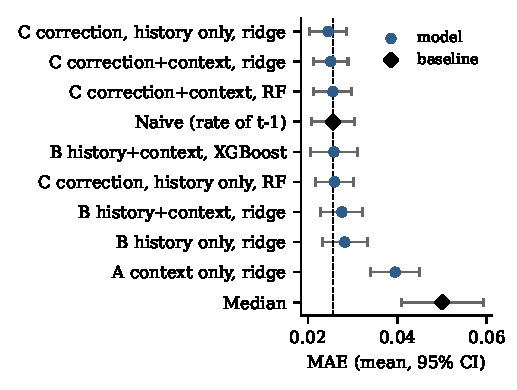
\includegraphics[width=\columnwidth]{fig_task1.pdf}
\caption{Task 1 MAE with 95\% corrected confidence intervals. The dashed line is the naive forecast.}
\label{fig:t1}
\end{figure}

Four findings stand out. \emph{Correcting beats predicting directly}: correction (C) improves the direct model (B) with the same inputs by 0.0037 MAE ($p_t<0.001$). \emph{Context adds nothing once history is known}: adding context to the correction model changes MAE by $-0.0006$ ($p_t=0.136$); context helps only in the 34 rows without history. \emph{The $t-1$ rate is the most valuable input}: without it, the naive forecast loses 21.3\% of accuracy, and in that conservative scenario no model beats the lagged naive (best $+3.8\%$, $p_t=0.136$). \emph{The best gain is small}: with Bonferroni over eight comparisons, its $p_t$ rises to 0.349; Section~\ref{sec:robust} shows that it holds after nested tuning but not under every sensitivity check.

\section{Results: Task 2 (Cold-Start Estimation)}

No model beats the median by character $\times$ sector. Grouping the median by institution type already improves the global median by 19.1\% (MAE 0.0405 vs.\ 0.0501), and the best model adds only 2.2\%, significant in Wilcoxon but not in the corrected test (Table~\ref{tab:t2}).

\begin{table}[!t]
\caption{Task 2 confirmation: $5\times5$ grouped CV, seeds 201--205}
\label{tab:t2}
\centering\footnotesize
\setlength{\tabcolsep}{3pt}
\begin{tabular}{@{}lcrcc@{}}
\toprule
Configuration & MAE [95\% CI] & Impr. & $p_W$ & $p_t$ \\
\midrule
Global median & 0.0501 [0.0425, 0.0577] & $-23.6\%$ & $<.001$ & $<.001$ \\
Median, char.$\times$sector & 0.0405 [0.0356, 0.0454] & -- & -- & -- \\
Ridge, MI & \textbf{0.0396} [0.0353, 0.0440] & $+2.2\%$ & .019 & .349 \\
Ridge, no reduction & 0.0399 [0.0356, 0.0443] & $+1.5\%$ & .113 & .562 \\
XGBoost, clusters & 0.0453 [0.0395, 0.0512] & $-11.8\%$ & $<.001$ & .066 \\
Ridge, PCA & 0.0454 [0.0380, 0.0528] & $-12.0\%$ & $<.001$ & .020 \\
Ridge, autoencoder & 0.0458 [0.0382, 0.0535] & $-13.1\%$ & $<.001$ & .014 \\
Ridge, kernel PCA & 0.0461 [0.0389, 0.0533] & $-13.8\%$ & $<.001$ & .005 \\
RF, clusters & 0.0478 [0.0428, 0.0528] & $-17.9\%$ & $<.001$ & .012 \\
\bottomrule
\multicolumn{5}{@{}p{0.95\columnwidth}@{}}{\scriptsize All models use the logit target; MI: mutual-information selection. With Bonferroni over seven comparisons the best $p_t$ becomes 1.0.}
\end{tabular}
\end{table}

\begin{figure}[!t]
\centering
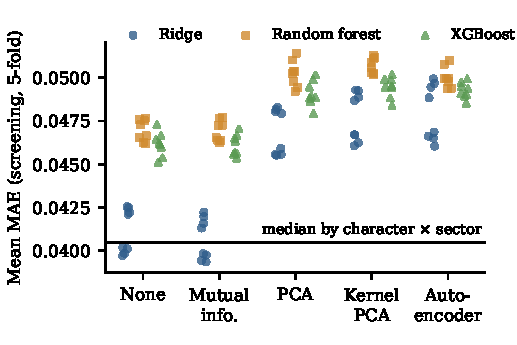
\includegraphics[width=\columnwidth]{fig_task2.pdf}
\caption{Task 2 screening: mean MAE of the 120 configurations by reduction method and model. The line is the median by character $\times$ sector.}
\label{fig:t2}
\end{figure}

The screening isolates the effect of each methodology, holding the other choices fixed (Fig.~\ref{fig:t2}). The logit target lowers MAE in 100\% of the pairs (mean $-0.0014$). Median and KNN imputation give the same mean MAE (0.0473). Mutual-information selection is neutral ($-0.0002$); PCA worsens MAE in every pair ($+0.0040$), and the nonlinear alternatives do not repair it (kernel PCA $+0.0045$, autoencoder $+0.0043$). In the confirmation, all three are significantly worse than no reduction ($p_t$ from 0.009 to 0.032). Cluster features have no effect (mean difference 0.0000). Ridge is the best model on average (0.0449), ahead of XGBoost (0.0480) and random forest (0.0490).

The K-means clusters ($k=6$, low silhouette) mostly separate cities, because territorial context is nearly constant within a municipality: Bogot\'a; large cities led by Medell\'in and Barranquilla; high-coverage intermediate cities; Cali and Manizales; medium-high poverty cities such as Cartagena and C\'ucuta; and a high-poverty periphery such as Monter\'ia and Quibd\'o. Their median rates range only from 8.5\% to 11.4\%, which explains why cluster membership adds no predictive value.

\section{Robustness}\label{sec:robust}

\subsection{Nested Hyperparameter Search}
We tuned each final model with nested CV: an outer $5\times5$ grouped CV (seeds 301--305) and, inside each outer training set, a randomized search of 30 iterations over a 3-fold grouped CV (Table~\ref{tab:tune}). Tuning helps the tree models of Task~2 significantly ($p_t<0.001$): they go from worse than the group median to indistinguishable from it. In Task~1 the ridge correction remains the only model that beats the naive forecast in both tests.

\begin{table}[!t]
\caption{Default vs.\ tuned MAE (nested CV, seeds 301--305)}
\label{tab:tune}
\centering\footnotesize
\setlength{\tabcolsep}{3pt}
\begin{tabular}{@{}clccc@{}}
\toprule
Task & Configuration & Default & Tuned & vs.\ baseline ($p_t$) \\
\midrule
1 & C, ridge & 0.0245 & 0.0245 & $+4.4\%$ (.011) \\
1 & C, random forest & 0.0257 & 0.0245 & $+4.3\%$ (.057) \\
1 & C, XGBoost & 0.0257 & 0.0250 & $+2.3\%$ (.359) \\
1 & B, XGBoost & 0.0258 & 0.0250 & $+2.6\%$ (.496) \\
2 & Ridge, MI & 0.0396 & 0.0396 & $+0.9\%$ (.596) \\
2 & XGBoost, clusters & 0.0448 & 0.0407 & $-1.7\%$ (.522) \\
2 & RF, clusters & 0.0469 & 0.0398 & $+0.4\%$ (.804) \\
\bottomrule
\end{tabular}
\end{table}

\subsection{Temporal Splits}
We trained on 2015--2017 and tested on 2018--2019 (pre-pandemic), and trained on 2015--2019 and tested on 2020--2021 (pandemic), re-tuning inside the training years. Task~1 is a one-step forecast: the observed rate of $t-1$ is used even when it falls in the test period. Intervals come from 1,000 bootstrap resamples of whole institutions. In all eight comparisons the 95\% interval of the difference between a tuned Task~1 model and the naive forecast includes zero. The naive forecast degrades least in the pandemic: MAE 0.0226 [0.0188, 0.0269] before and 0.0237 [0.0194, 0.0289] during ($\times1.05$), while the medians degrade $\times1.14$--$1.15$. The two splits train on 3 and 5 years, so each is compared only with its own baselines. Pooling the 1,095 test predictions of both splits, the naive forecast explains $R^2=0.61$ of the variance and the tuned ridge correction $R^2=0.66$; both are within 2 points of the observed rate in 68\% of the cases and within 5 points in 91--92\%, whereas the median by character $\times$ sector reaches $R^2=0.29$ and 39\% within 2 points.

The tuned ridge of Task~2 collapsed in the pre-pandemic split (MAE 0.0642 vs.\ 0.0360 with default settings; 0.0918 in 2019), with 39 of its 40 largest errors in Bogot\'a. A reproducible diagnosis traces it to one feature, municipal enrollment at $t-2$, which the weakly regularized tuned model ($\alpha=0.44$, 20 selected features) weighted heavily. Dropping that feature removes 83\% of the excess error, default regularization 31\%, and training only on years with observed SNIES data 48\%; clipping scaled features to $[-3,3]$ makes it worse, so the collapse is not extrapolation to extreme values. Grouped search within the training years cannot detect this kind of temporal instability; temporal validation can.

\subsection{Strict Cold Start by Municipality}
Grouping folds by municipality, so that no test city appears in training, leaves the conclusion intact: 0 of 7 configurations beat the group median (MAE 0.0373), and the best (XGBoost with clusters, 0.0375) differs by $-0.5\%$ ($p_t=0.902$). The fold containing Bogot\'a holds 38\% to 65\% of the test rows.

\section{Computational Complexity}

The cheapest models are also the most accurate here. With $n$ training rows, $p$ features, $T$ trees of depth $d$ and $k$ components, ridge costs $O(np^2+p^3)$ to fit, random forest $O(Tpn\log n)$, histogram XGBoost $O(Tdpn)$, PCA $O(np^2+p^3)$, kernel PCA $O(n^2p+n^3)$, K-means $O(Inkp)$ for $I$ iterations, and the autoencoder grows linearly with epochs, $n$, $p$ and hidden units. Table~\ref{tab:cost} reports measured costs on all 1,928 rows with one thread (Intel Core i5-12500H; median of five runs after a warm-up).

\begin{table}[!t]
\caption{Measured cost (one thread) and MAE of the final models}
\label{tab:cost}
\centering\footnotesize
\setlength{\tabcolsep}{3pt}
\begin{tabular}{@{}lrrc@{}}
\toprule
Model & Fit (ms) & Pred./1k rows (ms) & MAE \\
\midrule
T1 naive & 0.025 & 0.002 & 0.0256 \\
T1 ridge correction & 8.7 & 1.3 & 0.0245 \\
T1 XGBoost correction & 38.7 & 3.3 & 0.0250 \\
T1 XGBoost, hist.+ctx. & 146 & 6.1 & 0.0250 \\
T1 RF correction & 1,268 & 56.9 & 0.0245 \\
T2 group median & 0.53 & 0.25 & 0.0405 \\
T2 ridge + MI & 396 & 4.0 & 0.0396 \\
T2 XGBoost + clusters & 814 & 12.5 & 0.0407 \\
T2 RF + clusters & 1,368 & 18.9 & 0.0398 \\
\bottomrule
\end{tabular}
\end{table}

The best cost--error trade-off is the ridge correction in Task~1 and the group median in Task~2, about 725 times cheaper than the ridge model it ties with. Among preprocessing steps, the autoencoder is the slowest to fit (2.4~s), followed by kernel PCA (0.64~s); PCA takes 2.8~ms. Fitting on subsamples of 25\% to 100\% of the institutions gives empirical exponents in $n$ consistent with theory for kernel PCA ($2.37\pm0.19$) and KNN imputation ($1.83\pm0.03$); at these sizes fixed costs dominate the other methods. Extrapolating, kernel PCA would need about 10~hours and a 277~GiB kernel matrix with 100 times more rows, so neither it nor KNN imputation would scale to student-level data without approximations such as Nystr\"om features. The whole evaluation required 19,878 fits and 79 minutes on 16 threads; nested tuning accounts for 81\% of the fits.

\section{Bias and Limitations}\label{sec:bias}

The dataset represents HEIs with at least 100 enrolled students and consistent sources. Excluded rows have a median rate of 14.8\% vs.\ 9.9\% for included rows (25.7\% for excluded private HEIs), so results do not extend to small institutions or to military and police schools. Thirty-nine of 295 HEIs lack some of the seven years, and their median rate is higher (16.2\% vs.\ 9.6\%), so the complete panel overrepresents institutions that keep reporting. Bogot\'a, Medell\'in and Cali hold 49\% of the HEIs; territorial features barely vary within these cities, and their correlations with the rate change size and sign when the cities are removed. Only 24 technical and 37 technological HEIs exist, precisely the groups with the highest rates.

\emph{Measured error by subgroup.} No final model is worse than its baseline in any subgroup with an interval that excludes zero, except XGBoost in Task~2 in Bogot\'a (difference $-0.0036$ [$-0.0067$, $-0.0002$]). Errors are largest where data are thinnest: rows without history (Task~1 ridge 0.114, naive 0.127; 34 rows) and technical and technological HEIs (0.054--0.078).

\emph{Sensitivity.} Re-running the protocol without Bogot\'a (1,331 rows) or with 2017--2021 only (1,369 rows), the Task~1 ridge correction keeps its size ($+4.2\%$, $+4.3\%$) but loses significance ($p_t=0.097$, $0.117$). With a 200-student threshold, three models reach $p_t\approx0.04$, which would not survive a correction for the 20 scenario-by-model comparisons. Removing SENA changes nothing.

\emph{What the models use.} SHAP values and permutation importance agree on four of the top five features in both tasks. Task~1 models rely on the rates of $t-1$ and $t-2$ and the mean previous rate; Task~2 models rely on institution character and size, which is why the median by character $\times$ sector is so hard to beat. Territorial features weigh little and may mostly identify the city.

\emph{Other limitations.} We assume last year's rate is published when year $t$ starts; we did not verify this, so we report the conservative lagged scenario. Final hyperparameters are the consensus of the nested-search choices, which makes subgroup and sensitivity results slightly optimistic. Institution-level rates cannot identify which students drop out or why.

\section{Conclusions}

Institutional dropout in Colombia is highly persistent, and open territorial data add little to what an institution's type and its own history already say. With history, last year's rate is a strong forecast; a ridge model that corrects it improves MAE by about 4\%, but the gain is fragile under sensitivity checks, and no model is distinguishable from it in future years, including the pandemic. Without history, the median by character and sector is as good as any configuration we tested, including kernel PCA, an autoencoder and K-means cluster features; nonlinear reduction makes the estimates worse.

Two practical lessons follow. For forecasting, publishing each institution's latest rate early is worth more than any model we trained. For evaluation, grouping folds by entity, correcting for fold dependence and testing on later years are necessary: random splits and uncorrected tests would have reported gains that do not hold. Future work could add institution-level variables that open data lack, such as financial aid, faculty and programs, and student-level data where available.

\bibliographystyle{IEEEtran}
\bibliography{references}

\end{document}
